~~~~The problem of learning a BN given data $T$ consists of finding the BN that best fits the data $T$. In order to quantify the fitting of a BN a scoring function $\phi$ is considered.

Learning a Bayesian network is as follows:

Given a data $T = \{y_{1}, \cdots, y_{n}\}$ and a scoring function $\phi$, the problem of learning a Bayesian network is to find a Bayesian network $B \in B_{n}$ that maximizes the value $\phi(B, T)$.

Bayesian network structure learning algorithms can be grouped into two categories by Marco S. (2010).

\begin{description}

	\item[Constraint-based algorithms] These algorithms learn the network structure by analyzing the probabilistic relations entailed by the Markov property of Bayesian networks with conditional independence tests and then constructing a graph which satisfies the corresponding d-separation statements. The resulting models are often interpreted as causal models even when learned from observational data (Pearl J. 1988).
	
	\item[Score-based algorithms] The main idea behind score-based learning is to optimize the degree of match between the generated network and the observations. (Benjamin B. P., 2003) These algorithms assign a score to each candidate Bayesian network and try to maximize it with some heuristic search algorithm. The search problem of identifying a Bayesian network that has a relative posterior probability greater than a given constant is NP-complete. (D.M. Chickering, 1996) Greedy search algorithms (such as hill-climbing or TABU search) are a common choice, but almost any kind of search procedure can be used.
\end{description}

Traditionally, in searching for a Bayesian network structure, the set of states was the set of all possible Bayesian network structures, the representation was a Directed Acyclic Graph(DAG) and the set of operators were various small local changes to a DAG, e.g. adding, removing or reversing an arc, as illustrated in Figure 1.2. (R. Daly and Q. Shen., 2007)

\begin{figure}[!h]
	\centering
		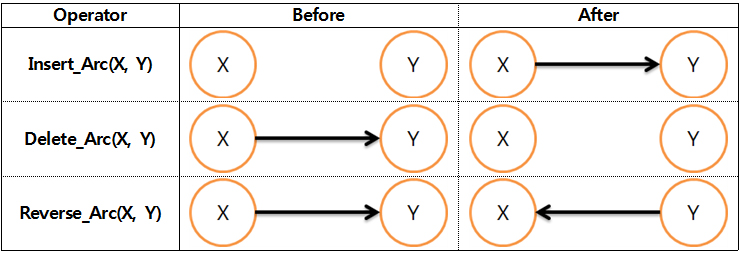
\includegraphics[height=100pt]{DAG_Operators}
		\caption{Basic Modification Operators in Searching for a Bayesian Network Structure}
\end{figure}	
